\chapter{Fairness} \label{chap:fairness}
% TODO: Introduction into the chapter, what we want to achieve, that we want try to define what Fairness is and how to measure it.

% TODO: Reword
So far, we have discussed recommender systems and the methods used in the field. We will step back and look at the problem from a broader perspective. Specifically, we want to focus on the importance of fairness and see how and if we can make group recommenders better if we understand it and define it properly.

We will start with a general introduction to the topic of fairness. Define its possible meanings and specify which one is important in our setting. This is required due to the overload of the word itself and the rising importance of the topic in today's world. Further, we will explain why fairness seems to be a crucial parameter in the group recommender setting and will try to reason about how to measure its effects.




\section{General} \label{sec:02_general}
% TODO: Start with a broad overview, why do we need something like fairness, define it, speak about it broadly.
% TODO: Problems with fairness, areas of usage, many possible definitions.

% I want to make an argument, that fairness is important to prevent notions of inequality which inherently leads to negative emotions

% it should lead the reader to think about it more, all the things we are discussing are general knowledge, we are not introducing something crazy

% IDEAS: Mention usage of the word fair/fairness
% https://www.youtube.com/watch?v=dKob6b8QzkU
% monkeys 
% https://www.youtube.com/watch?v=vHE6AYNOCrg
% many meaning of the word fairness, what does it mean for something to be fair

% the notion of fairness is probably important for developing cooperation

The word itself is very hard and controversial to define but in Cambridge Dictionary \cite{fairness_definition} it's defined as "The quality of treating people equally or in a way that is reasonable." Its use has been rising steadily from the 1960s as we can see on \ref{fig:popularity_of_fairness}.

\begin{figure}[htbp]
    \centering
    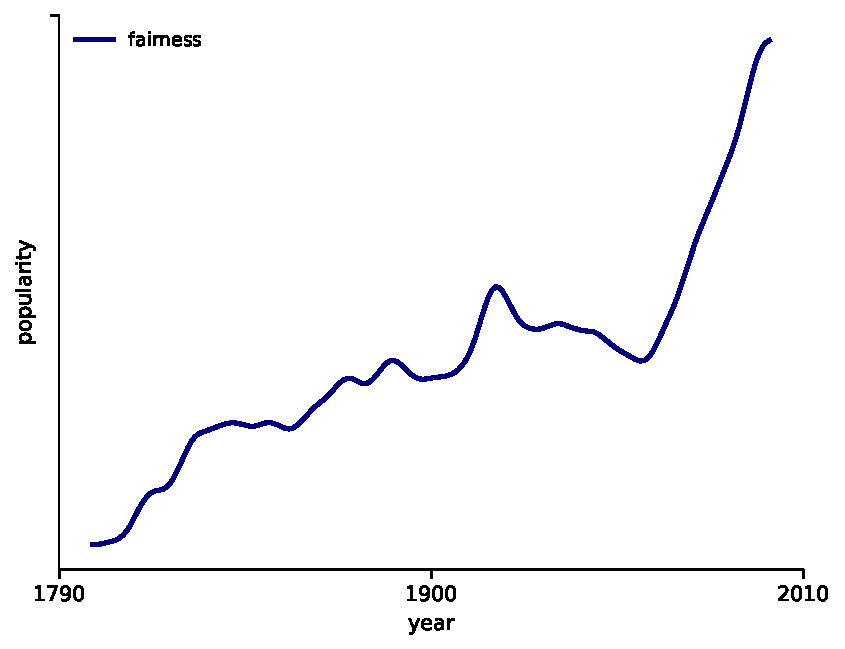
\includegraphics{img/google_ngram_fairness-eng_2012-1800-2000.pdf}
    \caption{The graph shows the phrase 'fairness' occurring in the corpus of English books from 1800 to 2010. Source: Google Ngram Viewer, corpora 2012. \cite{google_ngram_viewer_2012}}
    \label{fig:popularity_of_fairness}
\end{figure}

Humans are obsessed with fairness. From a young age, children will get sad when something is not fair, when their sibling gets a more significant piece of a pie, more attention from their parent, or any other unequal situation. It can induce strong emotions such as envy, sadness, or anger, and it emerges very early, as early as 12 months of age or sooner as researched in \cite{children_fairness}.

And this is not limited only to humans; we can observe the same behavior in monkeys. In \cite{brosnan2003monkeys}, the authors observed that if a monkey is getting the worse reward for the same task as its peer,  it refuses the reward and demands the same payout even if they were satisfied with the lesser reward for the same task before. In some sense, this is very strange, why should you care about someone having more if you have enough?

We observe the same behavior in many other species, but it does not hold for the animal kingdom in general. It seems that it requires a certain level of intelligence for the notion of fairness to emerge. As discussed in \cite{brosnan2014evolution}, based on studies of other non-human species, this evolutionary puzzle can be further dissected into responses to reward distribution among the cooperating group members. Where humans are even willing to seek equalization of outcomes even if it means that they will loose some of their own reward as studied in \cite{willing_to_pay_to_equality}. At the same time, we humans like "free-rides" where we get high rewards for a small amount of work but dislike when someone else gets the same. This directly corresponds with the fairness itself - "It is not fair if someone else gets something we don't.". But that all depends on our personality and the type of relationship involved. Some are, for example, willing to accept that your partner makes more. But that is very subjective and in some cases can lead even to a larger of envy involved.

\todo[inline]{Fairness acts as a group self healing property, where equality leads to more stable groups?}

In some cases we observe a pattern of generosity, where children are willing to make their own sacrifices in order to ensure fairness, so that the other person does not have less than them, as presented in \cite{children_generocity_blake}. The authors studied fairness in multiple cultural settings and found out that this behavior is learned and only present in some cultures.

On the other hand, our society widely accepts the notion of "winner takes all", which can be problematic in itself, for example, in sports and business. In business it directly shapes the distribution of wealth, which is considered one of the main problems of today's world. But discussing the social aspect of fairness is beyond the scope of this thesis.


When it comes to the true nature of fairness on the deepest level, it could even be possible that the notion of fairness emerges together with cooperation and therefore language and communication. It would mean that it is an inherent property of any intelligent agent that is created through an evolutionary process. But more research has to be done, as our understanding of intelligence, consciousness, and related hard to quantify phenomena is lacking.\newline

Let us now get back to fairness in the context of computer systems.









\section{Algorithmic fairness}\label{subsec:02_general.algorithmic_fairness_and_possible_meanings}
% The Emerging Theory of Algorithmic Fairness
We will focus on fairness regarding society or individuals interacting with a computer system. We will not discuss further any meaning of fairness outside of the domain of computer science. This topic steers away from the main goal of defining fairness for the group RS sub-domain, but we think that it is very important topic in general, deserves more spotlight and can be a good middle step to understand specifics of the group RS setting.

\subsection{How can computer be unfair?}
At first, the idea of a machine being unfair may feel strange. How can a computer that has no notion of race or ethnicity discriminate against a group of people? We say, that the algorithm is biased. In the end those who create the algorithms are people. Gathered data that are used to train the algorithm are from the real world. And so they reflect biases that are present in society. Algorithms with bias are not written with ill-fated purpose, it is just a side effect. We can say that the results of any machine learning (ML) algorithm are just the product of the underlying data. By design, accurate classifier will reproduce patterns found in training data.

It is important to define which sensitive characteristics need to be taken into account. That is a topic for social science to determine, but usually those are: gender, ethnicity, sexual orientation, disability, and so forth.

Research of algorithm fairness tries to analyze machine learning algorithms and data gathering and processing with the goal of understanding how bias in them is created and how it can be fixed.
\newline
As stated in \cite{pessach2020algorithmic_fairness} main sources of unfairness can be:
\begin{itemize}
    \item \textbf{Biases already included in the data set}\newline
    Such as dependence/correlation of data based on sensitive characteristics. Bias found in the data is by design reproduced by an accurate classifier.
    \item \textbf{Biases caused by missing data}\newline
    Results in data set that does not represent the target population.
    \item \textbf{Biases stemming from algorithmic objectives}\newline
    While training, we usually minimize some error, but that can lead to prioritization of interests of majority.
    \item \textbf{Biases caused by "proxy" attributes}\newline
    Some attributes that are not directly considered sensitive still can contain information from sensitive attributes. In other words, they are not independent. The algorithm can therefore use the "proxy" attribute and exploit the sensitive attribute indirectly.
\end{itemize}


In most of the recent literature fairness is studied from the perspective of discrimination and impacts of algorithms on society. We observe bias to specific groups of population based on their race, sex, nationality, education, beliefs, and many other attributes. And it is essential to study techniques and strategies to mitigate this unfairness.

Further, we can also view fairness from the aspect of algorithmic decision-making, where a decision process can introduce unfairness based on some non-deterministic property or computation. Some sectors such as justice and finance have to strive for equality of outcome due to the high cost of errors or unfair decisions. Either in the form of unjust punishments in the former case or financial loss in the latter one.


\subsection{Examples of algorithmic bias}\label{subsec:02_algo_fairness.examples_of_algo_biass}
We will now present a few instances of computer systems that have been used where bias towards a sensitive parameter had a substantial impact.

% https://towardsdatascience.com/what-is-algorithm-fairness-3182e161cf9f
% https://towardsdatascience.com/real-life-examples-of-discriminating-artificial-intelligence-cae395a90070

\begin{itemize}
    \item \textbf{Amazon's automatic recruiting system}\newline
    As reported by \cite{amazon-unfair-hiring-2018}, in 2018 it was found that new system for hiring people for Amazon was biased towards women. IT field being mostly male dominated - women represent only around 23\% as stated in \cite{women-in-tech-2021}. Due to this disproportion the algorithm discovered in training data pattern between gender of the candidate and hiring results which lead it to assume that male candidates are preferred before female ones. The algorithm was not told the gender of the candidate, but it inferred it from other data such as university, hobbies and other. This bias is a combination of "bias already included in the data set" and "biases caused by proxy attributes". The company later disbanded the team and left the tool only as a helper tool that works in conjunction with the recruiters, instead of solely automatically.
    
    \item \textbf{Apple's credit card}\newline
    Apple released it's own credit card in 2019. It works by you signing up for the service and the provider (Goldman Sachs) giving you credit limit based on some criteria. Some people, as reported in \cite{apple-card-washingtonpost-2019}, noticed that their wife was assigned smaller credit limit even though her credit score was higher and they only had one shared bank account.
    In this case, investigation by New York State Department of Financial Services came to conclusion based on an extensive analysis that no unlawful discrimination against applicants have taken place.
    
    \item \textbf{COMPAS} - Correctional Offender Management Profiling for Alternative Sanctions\newline
    COMPAS is an algorithm that was used in US justice system to predict the likelihood that a defendant would become a recidivist. Analysis \cite{compas-analysis-2020} found that black defendants were often predicted as being higher risk than they actually were and on the contrary white defendants were predicted to be less risky than in reality. In case of re-offended, this predicted risk was almost twice as high for blacks compared to whites. They conclude that the tool is very imprecise and does not reflect the true likelihood that it was designed to predict.
\end{itemize}

In these cases, society and mainly law has to act and protect those that are treated unfairly. European law can act as a good example of what can be done. The general data protection regulation (GDPR) and protection of individuals against algorithmic bias are some of the great and functioning examples.

Details about laws that are in effect in EU and definitions of sensitive characteristics and areas of protection can be found in Handbook on European non-discrimination law \cite{european-union-agency-for-fundamental-rights-2018}.


\subsection{Measures of algorithmic fairness}
It is necessary to 

We need to have a precise way how to measure bias of the sensitive characteristics. Some of the simple statistical methods directly sourced from \cite{wikipedia-algo-fairness} are:
\begin{itemize}


    \item \textbf{Independence}
        We say that sensitive characteristic S is independent of prediction R if:
        \begin{equation}
            P\left(R = r|S = a\right)=P\left(R=r|S=b\right) \quad \forall r\in R \quad \forall a,b \in S
        \end{equation}
    
    
    \item \textbf{Separation}
        We say that random variables $(R,A,Y)$ satisfy separation if the sensitive characteristics $A$ are statistically independent to the target value $Y$ given the prediction $R$.
        This relation can be expressed with:
        \begin{equation}
        \begin{split}
            P\left(Y=q|R=r,A=a\right)=P\left(Y=q|R=r,A=b\right) \\
            \quad \forall r\in R\quad q \in Y \quad \forall a,b \in A
        \end{split}
        \end{equation}
    
    
    \item \textbf{Sufficiency}
        We say the random variables $(R,A,Y)$ satisfy sufficiency if the sensitive characteristics $A$ are statistically independent to the target value $Y$ given the prediction $R$. This can be expressed as:
        \begin{equation}
        \begin{split}
            P\left(Y=q|R=r,A=a\right)=P\left(Y=q|R=r,A=b\right) \\
            \quad \forall q\in Y\quad r \in R \quad \forall a,b \in A
        \end{split}
        \end{equation}
    
\end{itemize}


The subsequent possible interpretation that applies to our group recommender domain is the notion of fairness in the sense of balance of preference between members of a group. Each member has their preference, and we are trying to balance them in the best possible way so that everyone likes the recommended object or list of objects equally. They may like the recommendation less because their favorite items may not be present.


\subsection{Other adverse effects}
% Zpracovat feedback loop, bias problemy muzou zpusobit problemy dlouhodobe, echochambers

We would now like to talk about other negative effect of not addressing the importance of fairness, when developing machine learning algorithms.

\subsubsection{Negative feedback loop}

A decision-making system that is learning from past data and is retrained in the future, will consume its own (previous versions') decisions as training data. This can lead to amplification of biases that were already present and to further skew the distribution of the underlying data. This effect is called "negative feedback loop".

In order to build robust and fair algorithmic systems, we need to understand when and why this effect emerges. When we look at it from a simpler perspective, where the current system deployed in production is just a set of predictions, then training the next model is just training the previous with additional data that the current model made (the set of predictions from production). In this sense the set of features selected while the current model was trained will correlate with the new data and therefore affect the selected and used features in the new training. This can be very detrimental to performance of the model. And it is not easily fixable due to how data is gathered and how machine learning is iterated.

We will mention an example from \cite{towardsdatascience_negative_feedback_loop}. Lets assume that we are building a decision-making algorithm that decides where to put our call-center capacity in order to generate the most profit. In other words, to which telephone numbers from some candidate list to call. And lets again assume that in the prior data the conversion rate of person coming from page X is 5\%, from page Y is 2\% and from page Z is 1\%. The algorithm will naturally be selecting to focus our capacity to X, because it has the biggest conversion rate. Now fast forward some time when we are retraining the model on new data. Due to us preferring the page X, and not calling to people coming from Y and Z our data distribution of conversion rate looks like this: X: 8.5\%, Y: 0.5\% and Z: 0\%. We end up having less data about Y and Z due to us, not calling people coming from those pages. Now we will retrain the model and this bias towards X will reinforce. In this way the performance of the model is decreasing, due to the data no longer following the actual underlying distribution. If we use ideas from Reinforcement learning - we are exploiting, but not exploring.

This negative feedback loop can be and is very detrimental to models' performance and in a wider view even dangerous to society. Which directly leads us to a second adverse effect of echo chambers.

\subsubsection{Echo chambers}
The feedback loop described in previous section can be observed in effect not only when retraining algorithms, but in social groups as well. People naturally seek out information that reinforce and support their existing views as stated in \cite{garrett2009_reinforcing_opinion}. Serving content to user that supports their views will therefore lead to higher satisfaction and interaction with the system. Together with metrics that are used while training content recommendation systems, which try to maximize the amount of time user spent interacting with the service, or return rate of the visitors, can lead to a creation of system that naturally locks its users in so called "echo chambers". While being inside, your own views will be reinforced. This, together with people increasingly consuming social media feed as their main source of news is probably one of the main forces behind the increasing polarization in society. But more research and empirical findings that directly support these assumptions is needed.
%\todo[inline]{Extend}
% Need to find source for the increasing polarization.









%\subsection{X}\label{subsec:02_general.x}


\section{Fairness in Group recommender systems} \label{sec:02_fairness_in_grs}
% TODO: Important to distinguish and define the fairness in the group setting. Other related things such as group dynamics, LONG-TERM fairness, balancing among users. Possible RS related problems.

% Already mentioned in the next chapter, need support for: single item vs list fairness.

%Equality of oportunity and equality of outocme a rozlisit mezi tim a my jdeme po oportunity of outcome, tam nejde tolik o bias ale o ten vysledek

So far, we have discussed algorithmic fairness in the context of equality of opportunity, where the main goal is to not discriminate against an individual. The same issues are present in the Group RS domain, but we will focus on equality of outcome more. Our objective is to fairly distribute item recommendation quality between group members, so that everyone is as satisfied as possible and satisfied equally.


\subsection{Specific cases of fairness}
Let us now mention some of the main ways how fairness in this context can be understood and specific differences between the different ways.

\begin{itemize}
    \item \textbf{Fairness distribution in isolated recommendation}\newline
    We recommend a list of items (possibly even a single item) and have to balance the items that all members will be satisfied by the selection. This single list is an isolated recommendation. We can view fairness in this setting as a direct optimization problem, where items are considered better if they are liked on average (among the group members) more than items liked by some part of the group and disliked by the other. As the group size grows, this is harder and harder to satisfy because a larger group will most probably have a broader preference which will be harder to satisfy.
    
    \item \textbf{Fairness in a list of items that are consumed sequentially}
    This setting differs from the previous because we can be recommending items that are less universally likable but more specific and liked by part of the group. Therefore intertwining the items so that each member will be satisfied "at some point". The balance of group-likable or member-likable items can be tuned according to the specific requirement.
    
    \item \textbf{Long-term fairness}\newline
    Further, we can distinguish another case where recommendations are provided in batches separated by some more significant amount of time (days or longer). This case is somewhat similar to the last one but differs by the fact that unfairness can be more costly to repair. If a person dislikes the item recommended by a group RS, they will less likely be part of the recommendation in the future. So the balance mentioned in the previous setting is an even more important and sensitive parameter to tune. And at the same time, it is more important to gather and process feedback.
    
    \item \textbf{Uneven importance of the group members}
    In some cases, there will be a situation where the expectation of fairness is distributed non-uniformly. For example, when watching a movie with your kids, you probably care about the satisfaction of your kids more than your own. But at the same time, you want to take yourself into account too. In these cases, it is essential to view required fairness as a fluid parameter that can be modified and satisfied by uneven criteria towards group members.
    
% TODO: It is nice to see what we want, but in order to build algorithms and improve, we first need to know how to measure it. List possible ways of how to measure the fairness, mainly in regards to group recommenders. Then discuss about the evaluation on data. The exact process of processing the the training and testing. Define everything very precisely and rigorously.
    
\end{itemize}

\subsection{Evaluation} \label{sec:02_evaluation}
\todo[inline]{DEADLINE 17.1. osnova v bodech}

% omezena komodita rozdistribuovat mezi zdroje
% 1 mira ferovosti a 2 mira relevance
% lepsi pro nas mit vsichni min a stejne nez nekdo vic a ostatni min
% najit metriky ferovosti a zamyslet se nad tim co a jak

\section{Other properties} \label{sec:02_other_properties}
Let us now discuss some similar properties that are closely tied together with fairness in the general and algorithmic setting as it is helpful to have a wide overview of the problem while designing algorithms that optimize fairness. We can have a fair algorithm, but to what use it will be, if it recommends bad items that are disliked. Fairness, as well as most other parameters we are usually trying to optimise has to be part of a multi-criterion optimization, especially in the non-academia setting.

\subsection{Bias}
As already mentioned before, bias is an important harmful property that we are aiming to reduce. Examples of bias are all around us. Each person has at least some prejudice and false ideas about topics that they have no expertise in. It is therefore important that we actively try to broaden our minds and actively suppress these biases. Just then, we can truly become equal as individuals.

From the algorithmic view, bias is mostly introduced from the underlying data, that we are using as a training set. Sometimes these biases are even knowingly used to even generate profit. For example in marketing, where sex is a very good indicator of preference. A good question arises - where lies the line between fair usage and abuse? We don't know yet, but it seems that privacy and fairness will be gaining importance and therefore the question of how to get rid of bias will become more significant.


\subsection{Privacy}
We have to extend our definition of privacy to ML systems as well. It tries to model given underlying data and therefore can leak users' information that is present in the data. Some models are explicitly based on similarity between users. A great example can be user-based methods from recommenders systems that were described in subsection \ref{subsec:01_rec_sys.main_alg_approaches}. In user-based methods we first find users that are similar to our target user to whom we're generating a recommendation and then we recommend those items that the similar users liked and our user have not yet seen. It can inherently happen that this preference we are unknowingly exploiting can be considered private. In this approach lies the great strength of user-based methods, they can extract latent meaning from data that would stay otherwise hidden. But on the other hand it can lead to a breach of privacy. Another great example can be text processing systems that are taught on a huge corpi of diverse text ranging from books, private messages, code repositories and other sources. A good example is a coding assistant for generating suggestions called Github Copilot. After the release of an initial version, it was discovered that it leaks secret information from the code repositories that it was trained on as discussed in \cite{github_copilot_leaks_2} and \cite{github_copilot_leaks}. More specifically - API access keys. The issue was later mitigated with applying content filters that check for known secret data such as the already mentioned API access keys, emails, passwords and other personal data.

Other issues apart from private data propagation out of training data-sets to predictions of the models can be the gathering and usage of massive training data-sets it self. Fair use which is vaguely mentioned by almost all service providers that gather users data should be revised and brought up to standards of the 21st century. But as we all know - government regulations lag behind.

\subsection{Trust}
There are certain machine learning applications that require aiming to optimize trust than others. It directly corresponds with how high of an impact the provided algorithmic decision can have. We will put a system that recommends books to a way lower level of scrutiny than a system that recommends which medication or treatment should a person get. This direct proportion between the importance of machine learning output and potential personal loss needs to be taken into account while designing the systems. Sometimes even highly effective and correct outputs of a machine learning system can be dismissed only due to a lack of trust in the system. Then the effectivity of the system can diminish even if the training and testing data tells otherwise. Trust can be greatly increased when providing explanations accompanying the output of the system.

\subsection{Explainability}
Having a reasonable explanation as to why we are getting the result we are getting can greatly improve real-world effectiveness of the system. It can decrease negative reactions to a non-ideal prediction and make users more forgivable as stated in \cite{tintarev2007survey}. We provide two examples of how can such an explanation look like, first from Amazon book store \ref{fig:amazon_explain_book_recommendation} and second from Facebook's explanation of why was a particular advertisement served \ref{fig:facebook_explain_book_recommendation}.

Explanations can achieve not only increased trust in the system as mentioned before, but increase in transparency, scrutability, persuasiveness, overall satisfaction and other positive effects. The main problem is, that they are generally hard to provide and they need to be taken into account while developing machine learning systems in all stages. Some algorithms are currently outright impossible to explain. One of the proliferated example of neural networks. Neural nets keep context in neural connections which are very hard to provide explanation for. We sometimes refer to this property of a system that we do not fully understand as 'black-box' systems. We know how they work, how to train them, but due to the inner complexity we fail to explain the exact way of how the result was calculated.

Explainability can be even indispensable. Lets for assume that a ML model is used to recommend a legal action against an individual in a judiciary setting. We cannot soundly present it as an evidence without being able to justify its actions and warrant its correctness.


\begin{figure}[htbp]
    \centering
    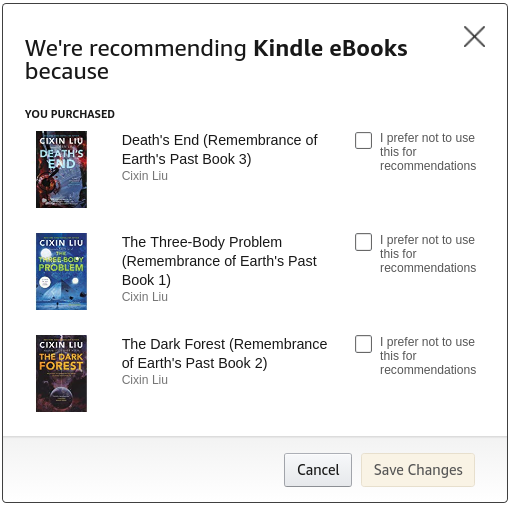
\includegraphics[scale=0.5]{img/AmazonExplanation.png}
    \caption{Amazon's web-page window that provides context why was a particular book recommended.}
    \label{fig:amazon_explain_book_recommendation}
\end{figure}

\begin{figure}[htbp]
    \centering
    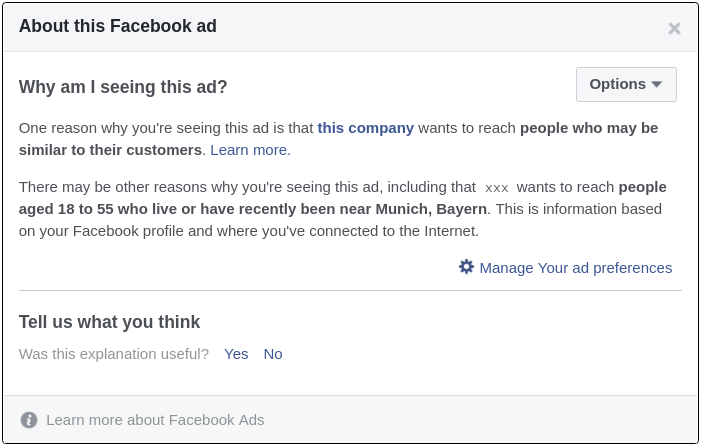
\includegraphics[scale=0.5]{img/FacebookAdExplanation2.png}
    \caption{Facebook's web-page window that provides information about what data lead to user's seeing Facebook's ads.}
    \label{fig:facebook_explain_book_recommendation}
\end{figure}

\subsection{Legitimacy}
Legitimacy can be viewed as an another step after explainability. If we provide a prediction together with a sound reasoning that can be repeated and verified either by a human analyst or by another trusted system, then we can use it in more serious and sensitive deployments. One of them can be the legal domain. In it computer systems can be used to provide unbiased and fair decisions and analysis if set up correctly. But as mentioned many times before, we need to be very careful with the data that we use for training. Lot of care needs to be taken even if we do not use an automated training solutions. Most of the current systems are most probably base on hand crafted rules that can very well be subject to bias as well. One of the examples being the system COMPAS presented in \ref{subsec:02_algo_fairness.examples_of_algo_biass}.

%\subsection{Auditability}
\todo[inline]{Add 'Auditability?'}

\subsection{Consistency}
We have different requirements for each of the ML systems. Some of them should aim to provide novelty, but for others it is important to stay consistent even for a slightly different input. Lets assume, that we are developing an illness detection algorithm, that offers the medical personal some insights about the patient based on provided symptoms. Then the predicted recommendation should not drastically change if for example the temperature changes by 0.1°C. It is therefore closely tied to the previous properties of legitimacy and explainability. Most high critical ML systems have to be designed with consistency in mind. Driver-less cars that abruptly change direction with only one pixel change in the input would not induce trust of its users.

From less high critical systems we can mention navigation properties in software and recommendation. We sometimes need machine learning user tailored systems that are exceptional for speeding up work or retrieval of information, but its users would not be comfortable with often changes in the provided recommendations. 

\subsection{Novelty}
But contrary to the previously mentioned consistency parameter, we sometimes strive for novelty and exploration. If a person is picking out a movie to watch, then showing them the same selection over and over would most certainly lead to their dissatisfaction due to the limited and repeated content that the system is providing. This property is most sought for in domains where exploration is important.

\subsection{Coverage}
\subsection{Diversity}

\subsection{Similarity}
\subsection{Accuracy}
\subsection{Precision}




% TODO: Fairness is not the only property we can try to manage, what about privacy, accuracy, precision, coverage, diversity, novelty and so on. Mention them first in an overview, then separately in subsections in more detail. Try to define them mathematically.
